\documentclass[russian]{article}
\usepackage[T1]{fontenc}
\usepackage[utf8]{inputenc}
\usepackage{geometry}
\geometry{verbose,tmargin=2cm,bmargin=2cm,lmargin=1cm,rmargin=1cm}
\usepackage{float}
\usepackage{textcomp}
\usepackage{amssymb}
\usepackage{graphicx}
\usepackage{babel}
\usepackage[T2A]{fontenc}

\makeatletter
\@ifundefined{date}{}{\date{}}


\begin{document}

\title{Теория графов. HW\#5}
\author{Тураев Тимур, 504 (SE)}

\maketitle

\paragraph{6.3} \textit{Возьмем $n$ вершин и расставим их равномерно по кругу. Зафиксируем некоторое четное натуральное число $k$ и проведем из любой вершины $k$ ребер, соединив эту вершину с $k/2$ вершинами слева по кругу от нее и с $k/2$ вершинами справа по кругу от нее. В результате получим $k$-регулярный граф, построенный на $n$ вершинах. Доказать, что для такого графа $\kappa(G) = k$}

Очевидно, что удаление $k$ вершин-соседей какой-либо вершины сделаем граф несвязным.
Докажем, что удаление любых $k-1$ вершины оставит граф связным. Выделим такие $k-1$ вершину в множество $S$: $|S| = k-1$.

Выделим какие-нибудь 2 вершины $u$ и $v$ в графе $G-S$. В изначальном графе между этими вершинами существовало 2 пути: по часовой стрелке по внешнему циклу и против часовой. Пусть $P_1$ и $P_2$ соответственно набор внутренних вершин в этих путях в изначальном графе.

Заметим, что по принципу Дирихле найдется такой путь ($P_1$ или $P_2$) в котором $S$ удалило меньше, чем $k/2$ вершин (действительно: предположив обратное, получим, что $|S| \geqslant k/2 + k/2 = k$. Противоречие с тем, что $|S| = k-1$).

Так как в графе $G$ из каждой вершины выходило по $k/2$ ребер в каждую сторону, то удаление менее $k/2$ ребер из какой-либо стороны не может удалить все возможные пути в эту сторону. А это значит, что мы можем найти путь между вершинами $u$ и $v$ в графе $G-S$ через тот путь $P_1$ или $P_2$, где $S$ содержит меньше $k/2$ вершин.

\paragraph{6.6} \textit{Привести алгоритм построения графа $G$, у которого $\kappa(G) = \kappa, \lambda(G) = \lambda, \delta(G) = \delta$}

\begin{itemize}
\item Построим две копии графа $K_{\delta(G)+1}$ -- полные графы на $\delta(G)+1$ вершинах. Это сразу выполняет третье условие: $\delta(G) = \delta$

\item Выделим в левом полном графе $\kappa$ вершин, а в правом полном графе $\lambda$ вершин и проведем $\lambda$ ребер так, чтобы каждая выделенная вершина была концом хотя бы одного нового ребра.
\end{itemize}

Граф построен. Тот факт, что $\kappa \leqslant \lambda \leqslant \delta$ не портит нам выполнение третьего условия: всегда найдутся вершины в полных подграфах, из которых мы не проводим новые ребра.

Очевидно, что удаление $\lambda$ новых ребер, равно как и удаление $\kappa$ выделенных вершин левом полном подграфе делает граф несвязным.

И понятно, что меньших разделяющих множеств нет, так как слева и справа у нас полные подграфы, а для них все три числа ($\kappa(G), \lambda(G), \delta(G)$) равны $\delta$. И если мы удалим меньшее число ребер (или вершин), то связи между двумя полными графами сохранятся, равно как и сохранятся связности в этих частях.

\paragraph{6.7} \textit{Определить значения $\kappa(G), \lambda(G), \delta(G)$}

\paragraph{6.7a}

\begin{center}
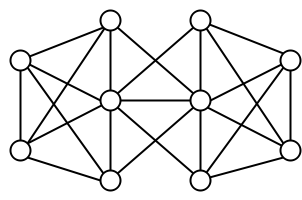
\includegraphics[scale=0.5]{6_7a_1.png}
\par\end{center}

Легко убедиться, что $\delta(G)=4$.

Также легко убедиться, что $\kappa(G)>1$. Приведем пример, показывающий,
что $\kappa=2$:

\begin{figure}[H]
\begin{minipage}[t]{0.5\columnwidth}%
\begin{center}
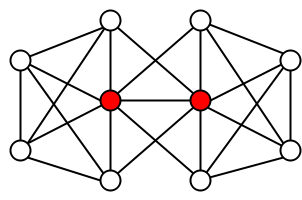
\includegraphics[scale=0.45]{6_7a_2.png}
\par\end{center}%
\end{minipage}\hfill{}%
\begin{minipage}[t]{0.5\columnwidth}%
\begin{center}
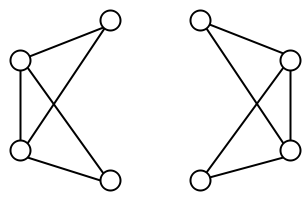
\includegraphics[scale=0.45]{6_7a_3.png}
\par\end{center}%
\end{minipage}\linebreak{}
\end{figure}


$\lambda(G)=4$ -- надо выбрать вершину со степенью равной 4 и удалить
все инцидентные ей ребра. Покажем, что реберная связность не меньше.

\begin{center}
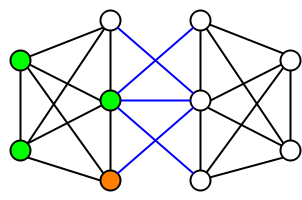
\includegraphics[scale=0.5]{6_7a_4.png}
\par\end{center}

Попробуем нарушить связность, удалив 3 ребра. Очевидно, что если пытаться
удалять средние ребра (покрашены в синий цвет), то потребуется удалить
5 ребер. Значит, их удалять смысла не имеет и следует пытаться нарушить
связность внутри одного из пятиугольников. Т.к. граф симметричный
-- выберем левый пятиугольник. Рассмотрим нижние четыре вершины (три
зеленые и одну оранжевую). Они образуют полный подграф $K_4$. Его реберная связность равна 3. При этом каждая из зеленых вершин соединена ребром с пятой вершиной пятиугольника. Следовательно, удалять имеет смысл только
три ребра, ведущие к оранжевой вершине. Но тогда граф все равно останется
связным. В силу симметрии то же верно и для верхних четырех вершин.
Следовательно, удалив 3 ребра, нарушить связность графа нельзя.


\paragraph{6.7b}

\begin{center}
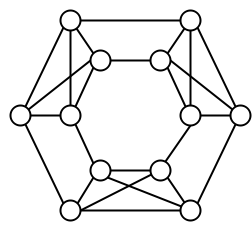
\includegraphics[scale=0.5]{6_7b_1.png}
\par\end{center}

Легко убедиться, что $\delta(G)=4$.

Покажем, что $\kappa(G)=4$. Удалим некоторое множество вершин и рассмотрим
получившийся граф. Рассмотрим в нем две несмежные вершины, значит
они и в исходном графе были несмежны. Рассмотрим возможные случаи
расположения вершин в исходном графе (пользуясь свойством симметрии
графа):

\begin{figure}[H]
\begin{minipage}[t]{0.5\columnwidth}%
\begin{center}
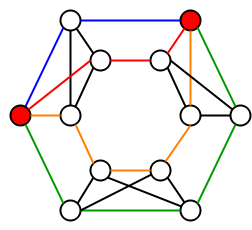
\includegraphics[scale=0.45]{6_7b_2.png}
\par\end{center}%
\end{minipage}\hfill{}%
\begin{minipage}[t]{0.5\columnwidth}%
\begin{center}
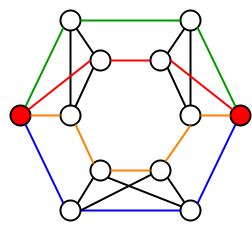
\includegraphics[scale=0.45]{6_7b_3.png}
\par\end{center}%
\end{minipage}\linebreak{}


\begin{minipage}[t]{0.5\columnwidth}%
\begin{center}
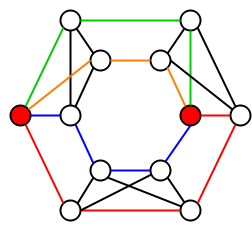
\includegraphics[scale=0.45]{6_7b_4.png}
\par\end{center}%
\end{minipage}\hfill{}%
\begin{minipage}[t]{0.5\columnwidth}%
\begin{center}
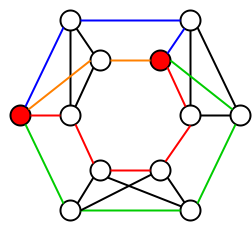
\includegraphics[scale=0.45]{6_7b_5.png}
\par\end{center}%
\end{minipage}
\end{figure}


Видно, что всегда существует четыре, непересекающихся по вершинам,
пути. Следовательно, чтобы сделать граф несвязным, необходимо удалить
не менее четырех вершин. Следовательно, $\kappa(G)=4$.

Из цепочки неравенств $4=\kappa(G)\leqslant\lambda(G)\leqslant\delta(G)=4$
следует, что $\lambda(G)=4$.

\paragraph{6.8} \textit{Доказать, что для любого 3-регулярного графа $G$ реберная и вершинная связность совпадают.}

Рассмотрим $S$ - минимальное вершинное разделяющее множество: $|S| = \kappa(G)$. Так как $\kappa(G) \leqslant \lambda(G)$, достаточно указать такое $F$ -- реберно-разделяющее множество -- чтобы $|F| = |S|$. Рассмотрим две компоненты связности $G_1$ и $G_2$, которые получатся после удаления из графа $G$ вершин из $S$. 

Заметим, что так как множество $S$ - минимальное, то каждая вершина в $S$ должна быть соединена хотя бы с одной вершиной из $G_1$ и $G_2$.

Так как граф 3-регулярный, то возможны несколько вариантов:

\begin{center}
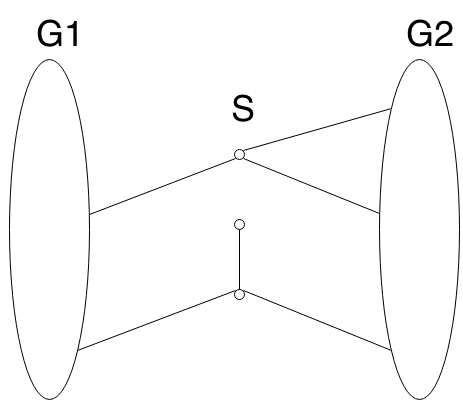
\includegraphics[scale=0.5]{6_8.png}
\par\end{center}

\begin{itemize}

\item Вершина $v$ из $S$ связана равно с одной вершиной из одной компоненты связности и ровно с двумя из другой (как верхняя вершина на рисунке)

Тогда удалим ребро, соединяющее вершину $v$ и ее соседа из $G_1$ (то есть разрушим путь из $G_1$ $G_2$ через вершину $v$)

\item Вершина $v$ из $S$ связана равно с одной вершиной из каждой компоненты связности и еще с одной вершиной $u \in S$ (нижняя вершинана рисунке).

В таком случае ясно, что ребра из вершины $u$ идут так же, как из вершины $v$. Удалим два ребра из вершин $u$ и $v$, идущие в одну из компонент связности, например $G_1$.
\end{itemize}

Получается, что удалением ровно $\kappa(G)$ ребер мы нарушили все пути, ведущие из $G_1$ в $G_2$, то есть предоставили реберно-разделяющее множество $F$, такое что $|F| = \kappa(G)$, то есть $\kappa(G) = \lambda(G)$

\paragraph{6.13} \textit{Доказать, что любой двусвязный граф $G$ допускает разложение $G$ на ручки, начинающиеся с произвольного цикла в этом графе.}

Пусть $G_0$ - произвольный цикл $C$ в графе.

Пусть $G_i$ - подграф, полученный после добавления в него $i$ ручек. Если еще $G_i \neq G$, то выберем какое-нибудь ребро $(x,y)$, лежащее в графе $G_i$ и ребро $(u, v)$, в этом подграфе не лежащее. Так как граф двусвязный, то эти два ребра лежат в одном цикле $C'$. Выберем из этого цикла путь $P$, который содержит ребро $(u, v)$ и ровно две вершины из $G_i$: они будут концами этого пути $P$. Теперь этот путь может быть добавлен к графу $G_i$ -- получим больший граф $G_{i+1}$, в котором $P$ -- это ручка.

Этот процесс обязательно закончится, причем тогда, когда он охватит все ребра в графе, так как на каждой итерации в $G_k$ добавялется по крайней мере одно ребро.

\paragraph{6.16} \textit{Доказать, что граф допускает сильную ориентацию тогда и только тогда, когда он реберно-двусвязен.}

\begin{itemize}
\item \textbf{Необходимость}. 

Пусть граф допускает сильную ориентацию, тогда он, очевидно связен.

Предположим, в графе есть мост $(u, v)$ которое ориентировано из $u$ в $v$. Тогда в этой ориентации не существует пути из $v$ в $u$. 

Таким образом, граф должен быть связным и не содержать мостов, то есть быть реберно-двусвязным.

\item \textbf{Достаточность}.

Пусть граф реберно-двусвязный. Тогда его можно разложить на ручки и замкнутые ручки начиная с произвольного цикла в этом графе.

Возьмем любой цикл в этом графе и ориентируем его <<по кругу>>, превратив его в сильно связный граф. Далее, при добавлении любой ручки, будем ее ориентировать всегда в одну сторону, последовательно. Если мы докажем, что добавление ориентированной ручки к сильносвязному графу сохраняет его сильносвязность, то теорема доказана.

А это доказать просто: добавим ориентированную ручку к сильносвязному графу $H$. И пусть ручка <<крепится>> к графу $H$ за вершины $x$ и $y$. Рассмотрим 2 любые вершины $u$ и $v$. Возможны следующие случаи:

\begin{itemize}
\item Обе вершины $u$ и $v$ лежат в графе $H$. Тогда они достижимы друг из друга в силу сильносвязности графа $H$.

\item Обе вершины $u$ и $v$ лежат на ручке, причем направление от $u$ к $v$. Тогда существует путь из $v$ в $u$: $v \rightarrow y \rightarrow x \rightarrow u$. Первая и третья стрелочки в силу ориентации ручки, вторая -- в силу сильной связности графа $H$.

\item Вершина $u$ лежит на ручке, а вершина $v$ в графе. Применяя аналогичные рассуждения приходим к выводу, что существует путь из $v$ в $u$: $v \rightarrow x \rightarrow u$ и существует путь из $u$ в $v$: $u \rightarrow y \rightarrow v$. 
\end{itemize}

Значит, добавление ориентированной ручки к сильносвязному графу сохраняет его сильносвязность

Теорема доказана.
\end{itemize}
\end{document}
